%===========================================================
% 01_overview.tex - 判断题识别概述
%===========================================================
\section{判断题识别概述}

\begin{frame}{判断题的特点}
    \textbf{常见符号类型:}
    \begin{columns}
        \column{0.5\textwidth}
        \begin{itemize}
            \item $\checkmark$(对号/正确)
            \item $\times$(错号/错误)
            \item $\sqrt{}$(根号/正确)
            \item $\bigcirc$(圆圈/正确)
        \end{itemize}

        \column{0.5\textwidth}
        \begin{center}
        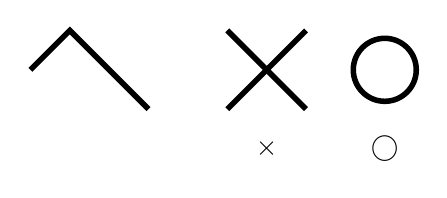
\begin{tikzpicture}
            \draw[line width=2pt] (0,0) -- (0.5,0.5) -- (1.5,-0.5);
            \node at (0.75,-1) {$\checkmark$};

            \draw[line width=2pt] (2.5,0.5) -- (3.5,-0.5);
            \draw[line width=2pt] (2.5,-0.5) -- (3.5,0.5);
            \node at (3,-1) {$\times$};

            \draw[line width=2pt] (4.5,0) circle (0.4cm);
            \node at (4.5,-1) {$\bigcirc$};
        \end{tikzpicture}
        \end{center}
    \end{columns}

    \vspace{0.5cm}

    \textbf{与选择题的本质区别:}
    \begin{itemize}
        \item 选择题:关注\textbf{填涂密度}(连续区域)
        \item 判断题:关注\textbf{符号形状}(笔画结构)
    \end{itemize}
\end{frame}

\begin{frame}{判断题识别的应用场景}
    \begin{columns}
        \column{0.5\textwidth}
        \begin{block}{教育考试}
            \begin{itemize}
                \item 标准化考试判断题
                \item 问卷调查判断题
                \item 课堂测验快速批改
            \end{itemize}
        \end{block}

        \column{0.5\textwidth}
        \begin{block}{其他场景}
            \begin{itemize}
                \item 表单勾选识别
                \item 质检合格/不合格标记
                \item 审批通过/驳回识别
            \end{itemize}
        \end{block}
    \end{columns}

    \vspace{0.5cm}

    \begin{alertblock}{技术挑战}
    \begin{itemize}
        \item 符号多样性:不同人书写习惯差异大
        \item 书写质量:笔画粗细、深浅不一
        \item 位置偏移:符号位置可能偏离预期
        \item 模糊符号:擦除修改留下的痕迹
    \end{itemize}
    \end{alertblock}
\end{frame}

\begin{frame}{识别方案对比}
    \begin{table}
        \centering
        \begin{tabular}{l|l|l}
        \toprule
        \textbf{方案} & \textbf{优点} & \textbf{缺点} \\
        \midrule
        轮廓特征法 & 速度快、无需训练 & 规则复杂、泛化弱 \\
        模板匹配法 & 简单直观、易于实现 & 对形变敏感、需要模板 \\
        机器学习 & 泛化能力强、准确率高 & 需要训练数据、计算复杂 \\
        深度学习 & 准确率最高 & 需要大量数据、资源消耗大 \\
        \bottomrule
        \end{tabular}
        \caption{判断题识别方案对比}
    \end{table}

    \vspace{0.3cm}

    \textbf{本周学习策略:}
    \begin{enumerate}
        \item 先掌握轮廓特征法(理解形状本质)
        \item 再学习模板匹配法(了解经典方法)
        \item 了解机器学习方法(开阔技术视野)
    \end{enumerate}
\end{frame}

\begin{frame}{判断题识别流程}
    \begin{center}
    \begin{tikzpicture}[node distance=0.8cm]
        \node[draw, fill=blue!10, rectangle, rounded corners, text width=2cm, align=center] (1) {图像预处理};
        \node[draw, fill=yellow!10, rectangle, rounded corners, text width=2cm, align=center, right=of 1] (2) {符号区域定位};
        \node[draw, fill=green!10, rectangle, rounded corners, text width=2cm, align=center, right=of 2] (3) {符号图像提取};
        \node[draw, fill=orange!10, rectangle, rounded corners, text width=2cm, align=center, right=of 3] (4) {特征提取};
        \node[draw, fill=red!10, rectangle, rounded corners, text width=2cm, align=center, right=of 4] (5) {符号分类};
        \node[draw, fill=purple!10, rectangle, rounded corners, text width=2cm, align=center, right=of 5] (6) {结果输出};

        \draw[->] (1) -- (2);
        \draw[->] (2) -- (3);
        \draw[->] (3) -- (4);
        \draw[->] (4) -- (5);
        \draw[->] (5) -- (6);
    \end{tikzpicture}
    \end{center}

    \vspace{0.5cm}

    \textbf{关键步骤说明:}
    \begin{itemize}
        \item \textbf{符号区域定位}:找到判断题符号所在位置(类似选择题定位)
        \item \textbf{符号图像提取}:裁剪出单个符号的图像
        \item \textbf{特征提取}:计算符号的形状特征(重点)
        \item \textbf{符号分类}:根据特征判断是$\checkmark$还是$\times$
    \end{itemize}
\end{frame}
